\chapter{Experimental analysis}
We have shown that exchange transparency and the enforcement of exchange policies offer great potential
to defend against manipulators and free-riders. In this chapter we establish
how a practical system responds to manipulation attempts. More specifically we emulate honest agents,
manipulators and free-riders in small scale experiments. We can observe the behavior of the 
honest agents and find that strategic manipulators are detected and isolated. We show that honest agents who
execute our mechanism are able to effectively detect free-riding agents that do not share or do not verify their partners 
and ignore them for future interactions.

The rest of the chapter is structured as follows: we first give an overview of the software 
architecture. Then we explain the setup of the experiments and the types of strategic manipulation
that will be emulated. Finally we present the results of the experiments.

% In the previous chapters we have explored the problem of dissemination of information in distributed
% trust systems. We offered a solution in the form of our multichain based TrustChain architecture, extended 
% it with internal agent state transparency and designed a mechanism that prevents any free-riding on
% dissemination and validation of information on transactions. In this chapter we aim to prove the 
% properties of the mechanism and architecture by experimental analysis. We built a proof-of-concept
% software that fully implements the architecture and mechanism described in this work. It allows us 
% to run an emulation of an agent network and study the behavior of agents in the presence of strategic
% manipulators.

\section{Implementation}
The experiments are run on a standalone implementation of TrustChain with the mentioned extension
and exchange mechanism. The code is available through GitHub\footnote{https://github.com/jangerritharms/extended\_trustchain}.
The code is based on the TrustChain implementation of py-ipv8\footnote{https://github.com/tribler/py-ipv8}
another project that is developed in the context of BlockchainLab. The implementation is done in 
Python. The programming language was chosen as it allows for fast development,
offers many useful extensions and the py-ipv8 dependency is also written in Python. 

An overview of the architecture is given by the drawing in Figure \ref{fig:software_architecture}.

\begin{figure}[h!]
  \centering
  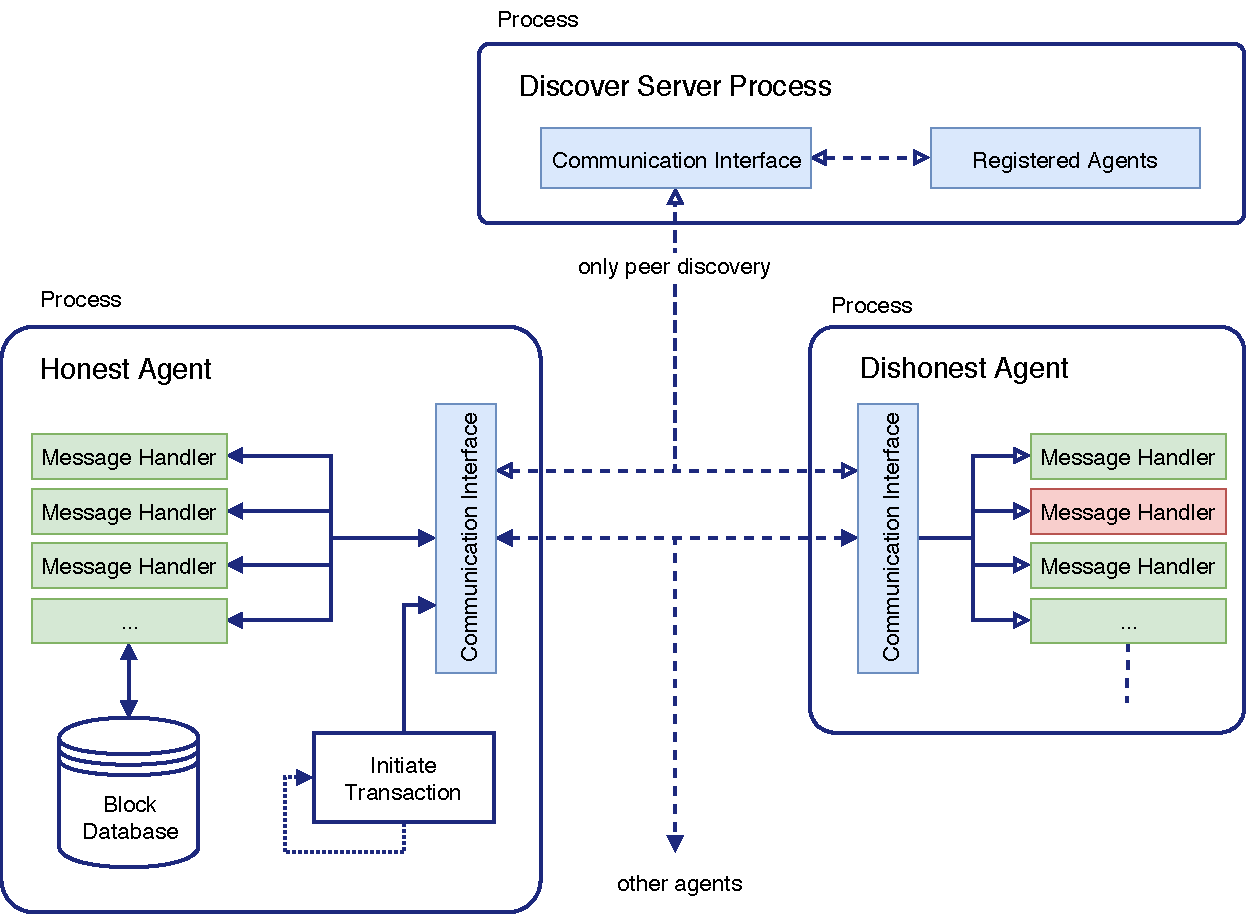
\includegraphics[width=0.8\textwidth]{images/architecture-2.pdf}
  \caption{Experiment setup and software architecture. Each agent runs in a separate process. The 
  main logic is inside the message handlers.}
  \label{fig:software_architecture}
\end{figure}

We run the experiments on a local machine. In order to emulate a distributed system, each agent 
runs in a separate process without any shared memory with other agent processes. Each agent runs 
their own database instance which stores the blocks. 

Agents communicate with each other through a communication interface. The interface 
provides an outgoing and incoming tcp port, implemented using the  \verb|zeromq| library. Messages
sent through the network as defined in the Google \verb|protobuf| format. 

The main logic of the agents is implemented in message handlers. Each message has a certain type,
for example a message to initiate an exchange or a message to reply to a block request. While all 
honest agents are handling messages in the same way, dishonest agents overwrite some correct 
message handlers with manipulated message handlers. 

Certain message handlers create blocks. The basic TrustChain block class and cryptography functions
are used from the \verb|py-ipv8| project. The blocks are stored in a MySQL database instance. The 
database interface also is used from the \verb|py-ipv8| project.

Next to the agents there is the discovery server which handles the peer discovery process. The 
experiment is started by spawning all agent processes and the discovery server. Once the agent 
process is started each agent sends a registering message to the discovery server to register the 
public key with the address of the tcp endpoint. After a 5 second initialization period it is assumed
that all processes have started and registered. The discovery server then sends a message to all 
registered agents containing their peers. Once that messages is received agents start running the
experiment. 

\section{Experiment design}
The goal of the experiments is to confirm our theoretical analysis of exchange policies from Chapter 
\ref{chap:model} and our architecture in Chapter \ref{sec:extension} in an experimental setup.
The following behaviors of agents will be analyzed in the experiments.

\begin{table}
    \caption{Agent types used in the experiments}
    \label{tab:agent_types}
    \begin{tabular}{p{4.0cm}|p{2.8cm}|p{7.6cm}} \toprule
    \textbf{Type} & \textbf{Sub-type} & \textbf{Behavior} \\ \midrule
    \multirow{2}{3cm}{Honest agents} & without auditing (default) & Exchanges and verifies agents normally \\ \cline{2-3}
    & with auditing & additionally replays the history of a peer to find any deviating behavior in the past \\ \midrule
    Exchange free-rider & - & Creates exchange blocks with empty exchanges \\ 
    % & Self-requests & Exchanges only own chain \\ \hline
    \midrule
    Verification free-rider & - & Acts honestly but blindly trusts all partners without verifying their data or behavior \\ \midrule
    \multirow{2}{3cm}{Manipulator } & Block withholder & Creates a normal transaction and tries to hide it afterwards \\ \cline{2-3}
    & Double-spender & Creates two conflicting transactions and shares them with two different peers \\ \bottomrule
    \end{tabular}
\end{table}

The honest agent without auditing only performs verifications of their direct exchanges. They do not
verify the complete history of their peers using the audit protocol. For some advanced attacks this
is necessary. We aim to show what additional verifications through the audit protocol can provide. 

Further we are interested in the ability to exclude free-riders that either do not exchange 
information or do not verify them. One way to ensure the consistency of the data in the network is 
to incentivize agents to share data and verify data. If all agents adhere to a certain exchange policy
this can be ensured. We analyze how honest agents react to agents that attempt to free-ride.

Finally we study two types of manipulating agents. A more complete list of manipulators is discussed
in Chapter \ref{chap:implementation}. In order to show that the mechanisms ensure the detection of 
manipulation we give two examples of manipulators: a block withholder, that is an agent who tries not 
share the complete chain, and a double spender, who forks his chain such that two transactions can 
be conducted while only recording one of them on the chain. If manipulation cannot be detected and
dealt with this endangers the validity of trust and reputation calculations because the underlying 
data could be invalid. We show that our system successfully detects and deals with manipulators.

% The goal of the experimental analysis is to show that free-riding on dissemination and validation of
% transaction information is no longer possible with the extension of TrustChain proposed in 
% chapter~\ref{chap:state_transparency} and the mechanism in chapter~\ref{chap:mechanism}. This would
% be a major step towards a secure and valid distributed trust system. 

The experiments are designed as follows.

\begin{itemize}
  \item \textbf{Network.} We emulate small networks of up to 6 agents, consisting of mixed sets of honest, free-riding and 
  malicious agents.
  \item \textbf{Peer discovery.} We assume that all agents are connected. This is implemented with the discovery server as described 
  above. 
  \item \textbf{Exchanges and interactions.} All agents are willing to interact. The initiation of an
  interaction is probabilistic with a expected frequency of 1 transaction every 5 seconds for each agent. 
  \item \textbf{Partner selection.} The partner selections is random with a uniform distribution. If 
  a exchange with the selected agent is already ongoing, no new interaction is initiated.
  \item \textbf{Handling of malicious agents and free-riders.} Any wrong behavior that is detected
  through a verification will be considered fraud. 
  \item \textbf{No forgiveness.} Honest agents do not forgive any wrong behavior.
  Once an honest agent detects a free-rider or malicious agent they will ignore any incoming requests
  and will not request interactions with them. 
  \item \textbf{No additional communication.} Agents only communicate to exchange blocks or create 
  transaction blocks. No information is shared on known malicious agents.
\end{itemize}


% In the experiments we emulate small networks of up to 6 agents. All agents are trying to perform 
% interactions with each other. The actual application domain is not modelled so transaction blocks 
% are empty. Agents are acting completely autonomously but know about all the other agents in the network. 
% At a frequency of 20 per second agents go through rounds, in each round an agent has a 1\% probability 
% of starting an interaction. This adds up to approximately 1 transaction every 5 seconds. In addition 
% agents respond to interaction requests from their peers asynchronously. 
% At the start of the interaction a partner is selected with uniform probability from all connected peers. If an interaction with 
% the selected partner is already ongoing, the new interaction request is cancelled without selecting a new partner. 

% Once the interaction is started honest agents perform exchanges and verification according the 
% mechanism as described in chapter \ref{chap:implementation}. The dishonest types of agents each have 
% some deviation from the expected behavior in order to obtain an unfair advantage. 
% All types of agents which were used in the experiments are listed in Table \ref{tab:agent_types}.
% , however we 
% implemented two types of manipulating behavior, block withholding and double spending.


\section{Experiment results}
In the following we will present the results of our experimental analysis.
\subsection{Dissemination free-riders}

% \begin{figure}
%     \centering
%     \begin{subfigure}{\textwidth}
%       \centering
%       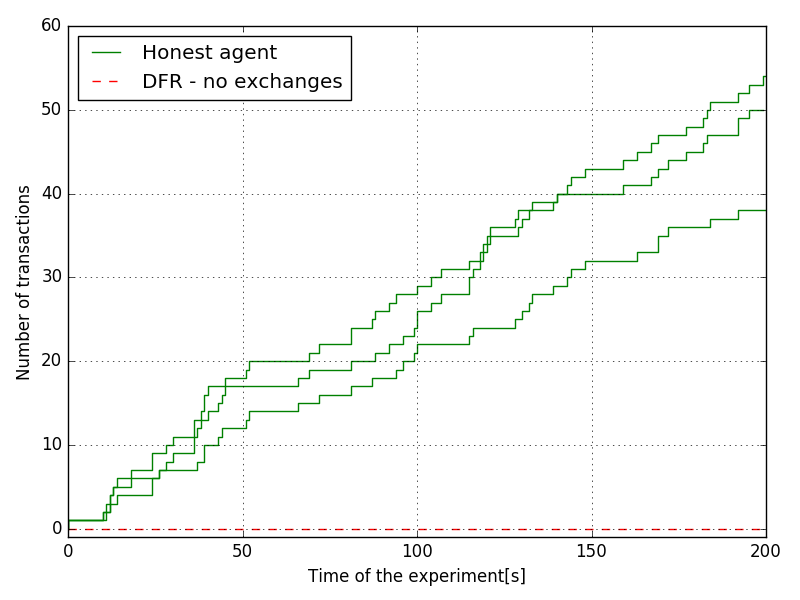
\includegraphics[width=.6\linewidth]{images/DFR_no_exchanges}
%       \caption{Transactions over time of honest agents with dissemination free-rider that does not 
%       perform any exchanges}
%       \label{fig:DFR_no_exchanges}
%     \end{subfigure}\\
%     \begin{subfigure}{\textwidth}
%       \centering
%       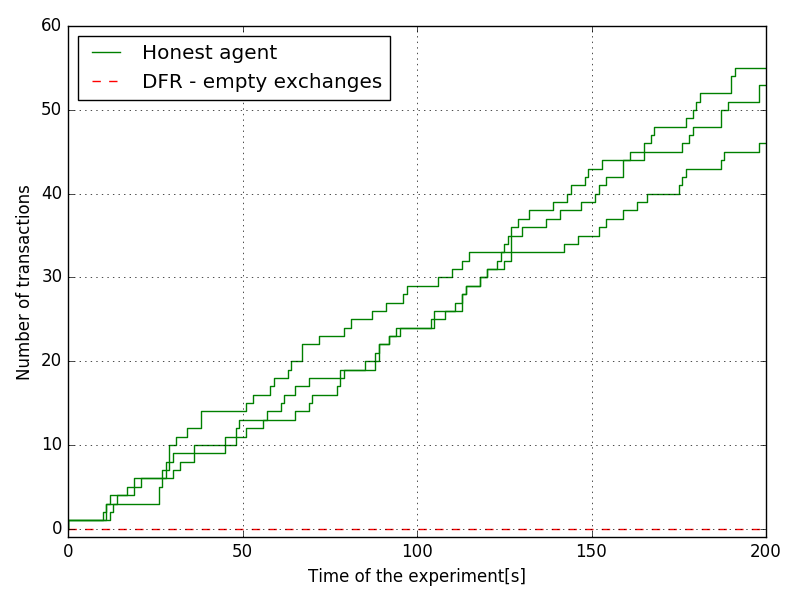
\includegraphics[width=.6\linewidth]{images/DFR_empty_exchanges}
%       \caption{Transactions over time of honest agents with dissemination free-rider that creates 
%       empty exchanges}
%       \label{fig:DFR_empty_exchanges}
%     \end{subfigure}\\
%     \begin{subfigure}{\textwidth}
%         \centering
%         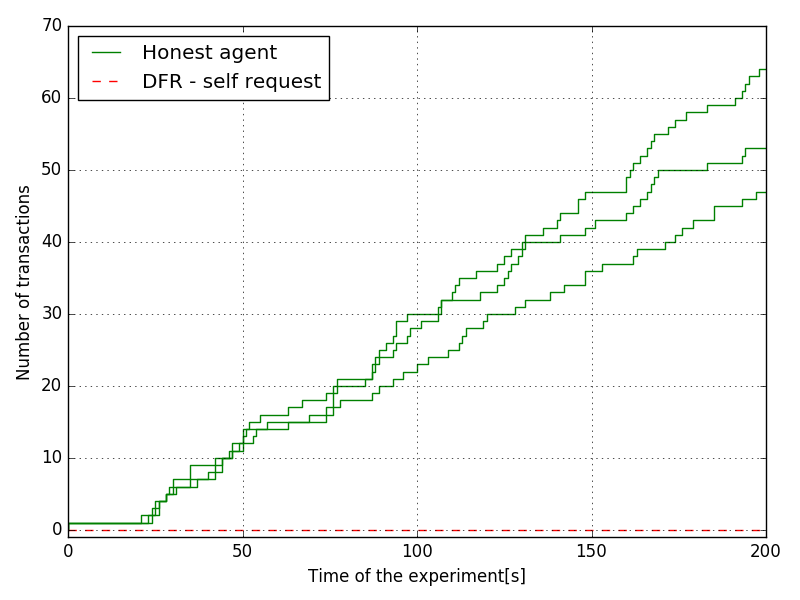
\includegraphics[width=.6\linewidth]{images/DFR_self_request}
%         \caption{Transactions over time of honest agents with dissemination free-rider that only 
%         exchanges own data}
%         \label{fig:DFR_self_request}
%       \end{subfigure}
%     \caption{Transactions over time of three experiments with different types of dissemination 
%     free-riders}
%     \label{fig:DFR}
% \end{figure}

Our first experiment analysis the performance of our exchange mechanism against free-riders. The 
exchange of information is vital against the double spend attack and other inconsistencies. An a
agent that does not exchange data is not able to provide any verification service to the network. If
this is a valid strategy more agents can free-ride, thus jeopardizing the network's security. It is 
one of our goals to stop free-riding behavior by creating a strong incentive to exchange. 
In order to secure the system, honest agents should be able to detect free-riders and ignore them.
This will remove any possible future profit from free-riders which should incentivize them to become honest.

In this first set of experiments we observe the behavior of three honest agents in the presence of 
a exchange free-rider that aims to create exchange blocks with empty exchanges. Therefore if an 
honest agent sends data the agent acts as if no data was received and puts an empty hash into the 
exchange blocks. At the same time the free-rider does not request any blocks from the partner.

Figure \ref{fig:DFR_no_exchanges} shows the number of transactions of each 
agent against the time of the experiment. All honest agents steadily increase their successful 
interactions throughout the experiment and end up between 40 to 60 transactions. The free-riding agent
is not able to perform a single interaction. That means all honest agents detected the free-rider 
as a dishonest agent and consequently ignored him. 

As expected, an agent has no chance to interact with the honest agents without a complete exchange. 
We have shown this property in Theorem \ref{thm:no_interaction}.


\begin{figure}
  \centering
  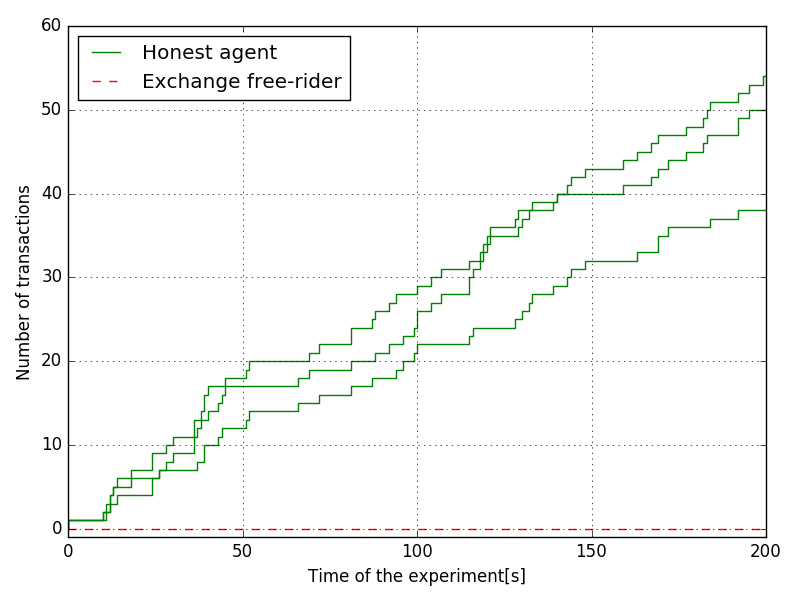
\includegraphics[width=.6\linewidth]{images/gossip_free-rider}
  \caption{Transactions over time of honest agents with exchange free-rider (both types give same result)}
  \label{fig:DFR_no_exchanges}
\end{figure}


% Finally, the third type of dissemination free-riders, results shown in Figure\ref{fig:DFR_self_request}
% , requests and sends data about itself but not any other knowledge. When in the responder position, 
% the agent can request only its own blocks. As initiator the agent tries to act again as if no data
% was received other than its own blocks. However the partner can see that the exchange block proposal
% does not properly represent the data exchanged and will therefore stop the transaction. Also this way
% the agent is not able to interact with honest partners. 

We find that dissemination free-riding leads to isolation and no transaction with honest partners. 
That means no reputation or trust will be build with this type of misbehaving agents and any hope for
future rewards is voided. Agents have to disseminate their data in order to be accepted and to prosper.

\subsection{Colluding free-riders}
Our second experiment analyses the impact of multiple free-riders in a collusion attack. In order to
be accepted as honest agents without gossiping, colluding agents can work together and sign empty exchanges for 
each other. This will create a seemingly valid history for the free-riders. Their goal is to interact 
with each other \textit{and} with the honest agents while exchanging less than necessary. Honest agents
should ignore them in order to keep their network safe and honest.

In order to analyze this situation we ran an experiment with three honest agents and three colluding gossip 
free-riders. The transactions are plotted against time in Figure \ref{fig:50percent}.

\begin{figure}[h!]
    \centering
    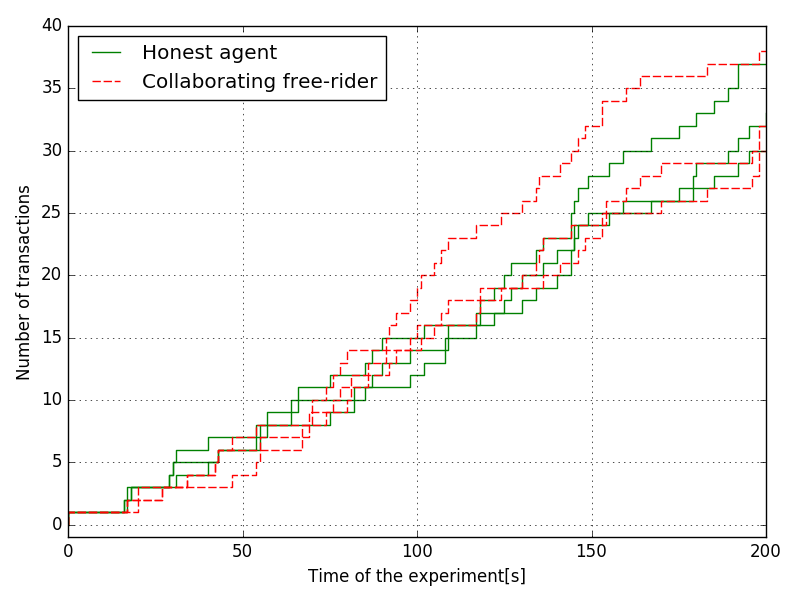
\includegraphics[width=0.7\textwidth]{images/50percent}
    \caption{Transaction history of three honest agents and three dissemination free-riders
    that are cooperating}
    \label{fig:50percent}
\end{figure}

\begin{figure}[h!]
    \centering
    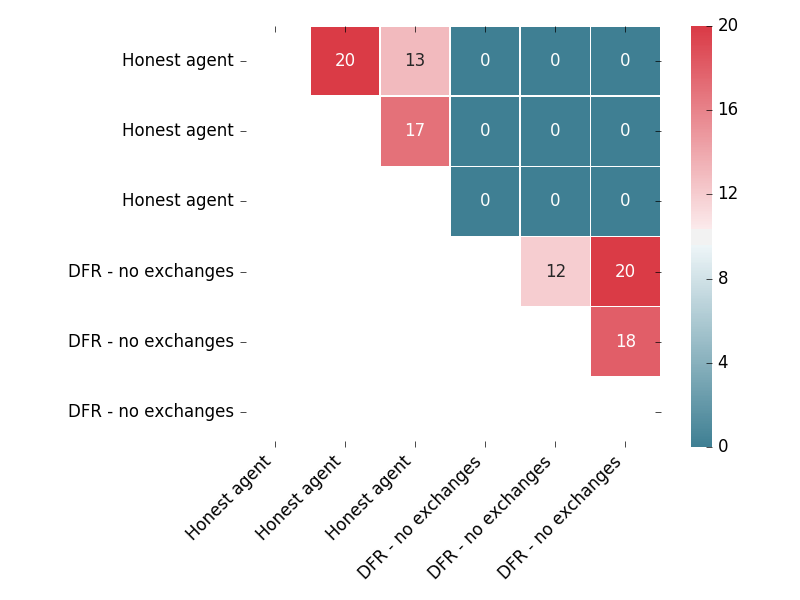
\includegraphics[width=0.8\textwidth]{images/50percent_interaction_matrix}
    \caption{Interaction matrix of quantifying the network separation}
    \label{fig:50percent_matrix}
\end{figure}

Again each line in the plot refers to the successful transactions of one agent. The plot shows six 
lines going almost in parallel which means that all agents fare equally well. However the plot does
not show which agents interact with each other. Therefore an interaction matrix is shown in Figure 
\ref{fig:50percent} which shows for each agent, how many interactions they had with each of their 
peers. 

From Figure \ref{fig:50percent_matrix} it becomes clear that no interactions (red squares) happen 
between honest and dishonest agents. Honest agents interact with honest agents, while dishonest
agents interact with dishonest agents. When dishonest agents try to interact with honest agents, 
honest agents will not sign an exchange block with empty hashes. So even though their history is 
correct according to the exchange policy, honest agents are still able to separate dishonest from
honest agents. This leads to network separation.

\subsection{Malicious behavior}
In the next experiment two types of malicious behaviors are analyzed: forking and block withholding. 
Similar to the free-riding, honest agents who use the TrustChain architecture and our exchange and 
verification mechanism should isolate the malicious agents. We have discussed that manipulation of 
the data the underlies reputation and trust calculation will invalidate the trust and reputation 
built in the system. It is therefore key to defend against manipulations.
The results of the experiments are 
presented in a similar format as previously in Figure \ref{fig:malicious}.

Both agents perform an attack with a 25\% chance in each round.
The transaction hider is able to obtain six successful interactions before all honest agents ignore him and the line flattens. When trying to withhold a block any honest agent is able to detect the fraud. The agent is not able to hide any transactions because any future partner expects the complete chain from that agent. Any missing blocks in the chain will be seen as a manipulation attempt.

The same can be observed for the double-spender. After the fork happens, the forking agent is detected by a partner 
once the partner receives the two conflicting blocks. Depending on the peer selection and the network size, this can 
take several rounds. Therefore the forking agent is able to perform 9 interactions in the first 20 
seconds of the experiment. After those interactions the red line indicating the forking agent 
flattens, meaning no more successful interactions happen. 

\begin{figure}
    \begin{subfigure}{\textwidth}
      \centering
      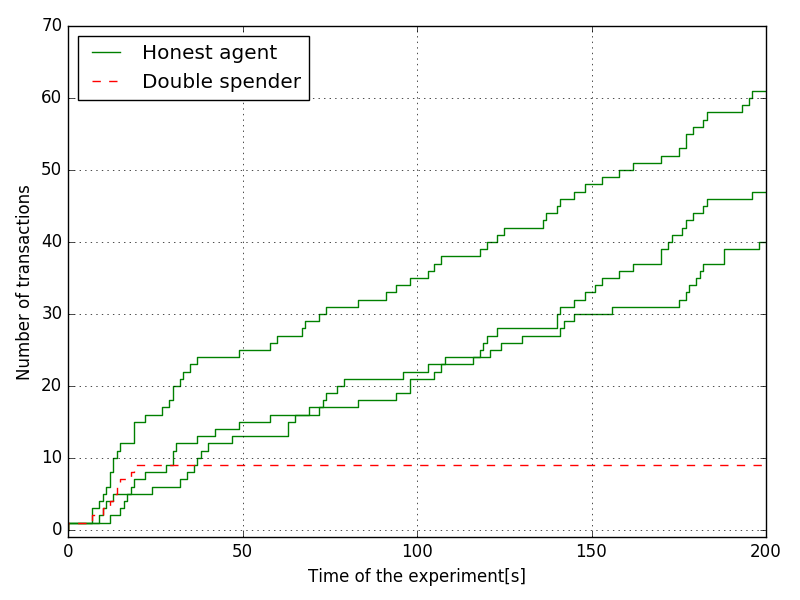
\includegraphics[width=.7\linewidth]{images/double_spending}
      \caption{Transaction history of three honest agents interacting with one strategic manipulator who performs a fork}
      \label{fig:forking}
    \end{subfigure}\\
    \begin{subfigure}{\textwidth}
      \centering
      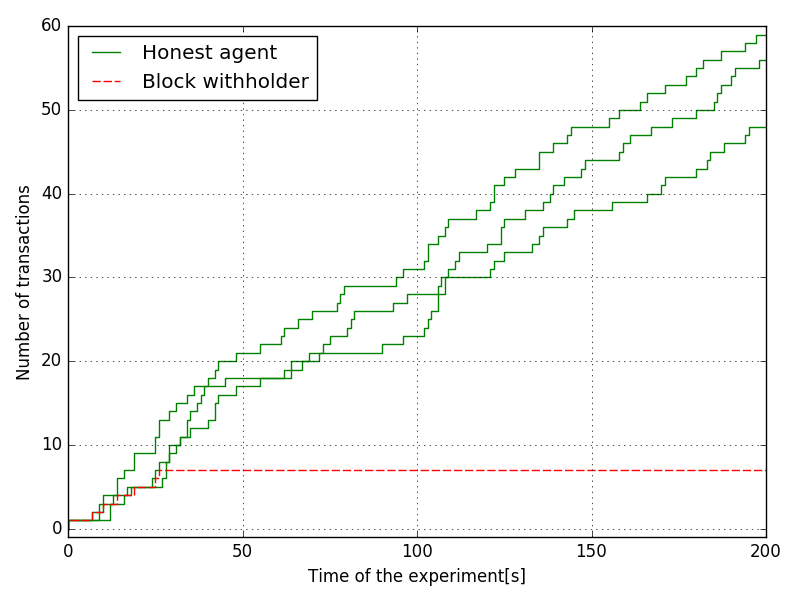
\includegraphics[width=.7\linewidth]{images/transaction_hiding}
      \caption{Transactions over time of three honest agents with one strategic manipulator who tries to hide a transaction}
      \label{fig:DFR_empty_exchanges}
    \end{subfigure}\\
    \caption{Experiments of honest agents with sinlge malicious agents}
    \label{fig:malicious}
\end{figure}

\subsection{Verification free-rider}
In the previous experiment we showed that malicious agents can be detected and isolated. In Chapter
\ref{chap:model} we have presented a theoretical study that shows that with the Network-State-Exchange
policy also those agents that knowingly interact with those malicious agents can
be isolated. This is possible \textit{auditing} the complete history of an agent and redoing the 
verifications. Any honest agent that obtains the full knowledge of the subject can perform this check 
ad find any failing verification which signals dishonest behavior.

In this experiment we study an combined attack. On the one hand a double-spender is creating a fork
in order to gain an advantage. On the other hand another agent does not perform any verifications
and interacts even when possibly knowing about a double spender. This is similar to the verification
free-rider and the double-spender colluding. The attack is difficult to detect because the agent
that does not perform verification acts completely honestly in all other regards.

We study two situations how honest agents behave in this situation, once without auditing, once with
auditing.

The results of the first case are presented in Figure \ref{fig:verification_doublespend_honest_combined}. 
The verification free-rider, represented by the blue dotted line in the figure is able to perform 
just as well as the honest agents. The forking agent is mostly ignored. The interaction matrix in 
Figure \ref{fig:verification_doublespend_honest_matrix} shows that most of the interactions of the 
forking agent come from the verification free-rider who does not perform any checks and therefore 
does not care about the fork.

\begin{figure}[h!]
    \begin{subfigure}{\textwidth}
      \centering
      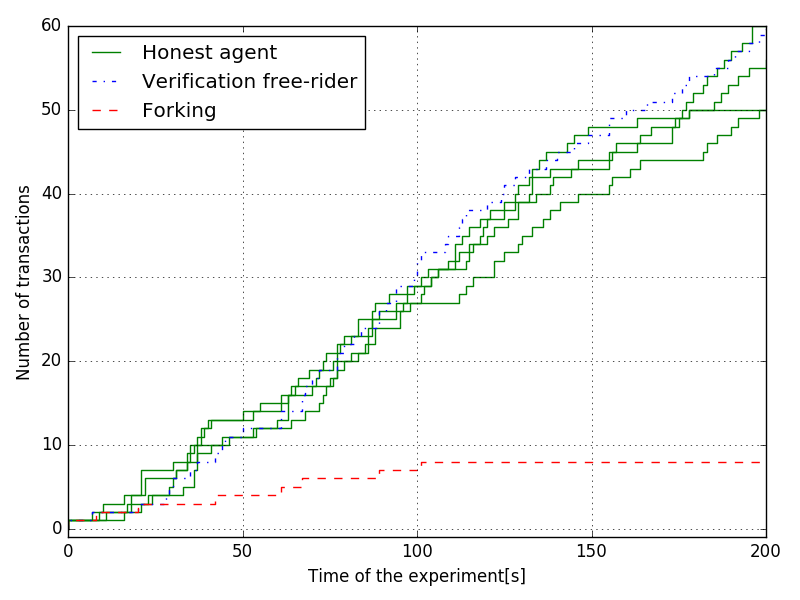
\includegraphics[width=.7\linewidth]{images/verification_doublespend_honest}
      \caption{Transaction history of three honest agents interacting with one strategic manipulator who performs a fork and a verification free-rider}
      \label{fig:verification_doublespend_honest}
    \end{subfigure}\\
    \begin{subfigure}{\textwidth}
      \centering
      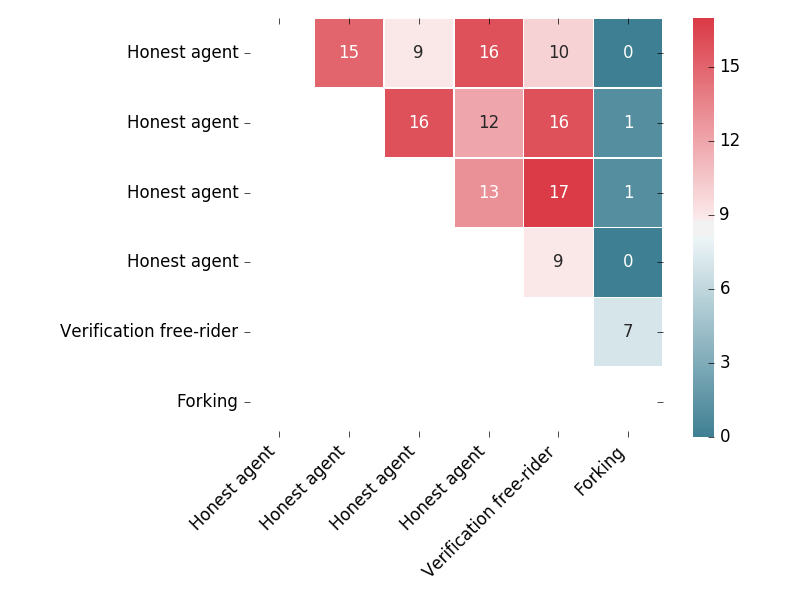
\includegraphics[width=0.8\textwidth]{images/verification_doublespend_honest_matrix}
      \caption{Interaction matrix of three honest agents with one strategic manipulator who performs a fork and a verification free-rider}
      \label{fig:verification_doublespend_honest_matrix}
    \end{subfigure}\\
    \caption{Experiment with three honest agents without replay verification, one malicious agent 
    and one verification free-rider}
    \label{fig:verification_doublespend_honest_combined}
\end{figure}

Next we repeated the experiment, but this time the honest agents perform auditing of their
partners before every interaction. The results are shown in Figure \ref{fig:verification_doublespend_combined}. 

The results show that after a long initial phase in which the blue and red curve seem to follow 
the green curves, they do get shallower after around 100 seconds. It is quite obvious, at least 
from the 100 second mark onwards, that the blue and red curve are running exactly in parallel. This is
because after detecting the forking agent and the verification free-rider, the honest agents are 
able to identify \textit{both} dishonest agents and ignore them for future interactions. Also the interaction
matrix shows that in the end, both dishonest agents get few interaction with the honest agents. 

\begin{figure}[h!]
    \begin{subfigure}{\textwidth}
      \centering
      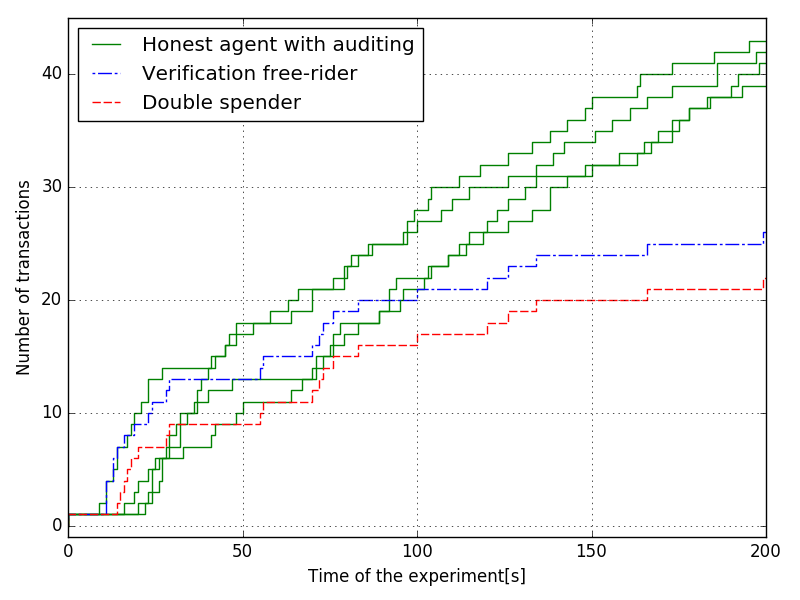
\includegraphics[width=.7\linewidth]{images/verification_doublespending}
      \caption{Transaction history of three honest agents with replay verification interacting with one strategic manipulator who performs a fork and a verification free-rider}
      \label{fig:verification_doublespending}
    \end{subfigure}\\
    \begin{subfigure}{\textwidth}
      \centering
      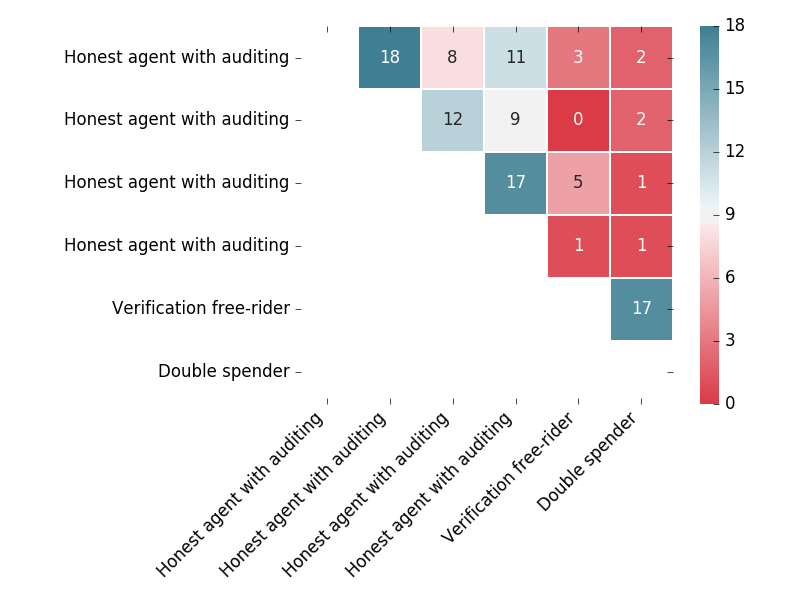
\includegraphics[width=.8\linewidth]{images/verification_doublespending_matrix}
      \caption{Interaction matrix of three honest agents with replay verification with one strategic manipulator who performs a fork and a verification free-rider}
      \label{fig:verification_doublespending_matrix}
    \end{subfigure}\\
    \caption{Experiment with three honest agents without replay verification, one malicious agent 
    and one verification free-rider}
    \label{fig:verification_doublespend_combined}
\end{figure}

\section{Chapter conclusion}
In this chapter we have studied the recording of exchanges and implementation of Network-State-Exchange
policy in an experimental setting. We have shown that any honest agent is able to ignore agents that
do not exchange correct data. Even if agents are working together they are not able to interact with
honest agents without exchanging the correct data and creating signed proof of that exchange. 

Even any previous collusion with a malicious agent can be found through proof-of-knowledge of a 
double spend on the verification free-rider's chain. We can conclude that the mechanism of recording
block exchanges enforces agents to obtain information and ignore any known malicious agents or 
become a fraud themselves.